\documentclass[aspectratio=169,11pt]{beamer}
\usetheme{default}
\usepackage[T1]{fontenc}
\usepackage[utf8]{inputenc}
\usepackage{booktabs}
\usepackage{array}
\usepackage{tikz}
\usetikzlibrary{positioning,arrows.meta}

\definecolor{midblue}{HTML}{1F5FAD}
\definecolor{softred}{HTML}{C0392B}
\setbeamercolor{frametitle}{fg=midblue}
\setbeamercolor{title}{fg=midblue}
\setbeamercolor{structure}{fg=midblue}
\setbeamercolor{alerted text}{fg=midblue}
\setbeamertemplate{navigation symbols}{}
\setbeamertemplate{footline}[frame number]
\setbeamertemplate{itemize items}[circle]

\newcommand{\hl}[1]{\textcolor{midblue}{\textbf{#1}}}
\newcommand{\story}[1]{\par\vspace{6pt}\small\textcolor{softred}{\textbf{What went wrong:}} #1}

\title{GraphRAG Explorer}
\subtitle{Discovering how Austrian banks, owners and regulators are connected}
\author{Kacper Zaleski}
\date{}

\begin{document}

%-------------------------------------------------------------
\begin{frame}
  \titlepage
\end{frame}

%-------------------------------------------------------------
\begin{frame}{The goal}
  \begin{itemize}
    \item A \hl{runnable app} where people \hl{visually explore} facts and connections they did not know
    \item From documents to a knowledge graph to an explorer UI, end to end
    \item Every fact \hl{traceable to its source passage}
    \item Plus the honest question: does the graph make \hl{answers} better than plain RAG?
  \end{itemize}
  \vspace{8pt}
  \small
  \begin{tabular}{ll}
    Corpus & 22 Wikipedia articles: Austrian banks, owners, regulators \\
    Stack & Python, FastAPI, Neo4j, React + Cytoscape.js, Docker \\
    LLMs & Gemini (free tier), switchable: Groq, Cerebras, Mistral \\
  \end{tabular}
\end{frame}

%-------------------------------------------------------------
\begin{frame}{Architecture}
  \centering
  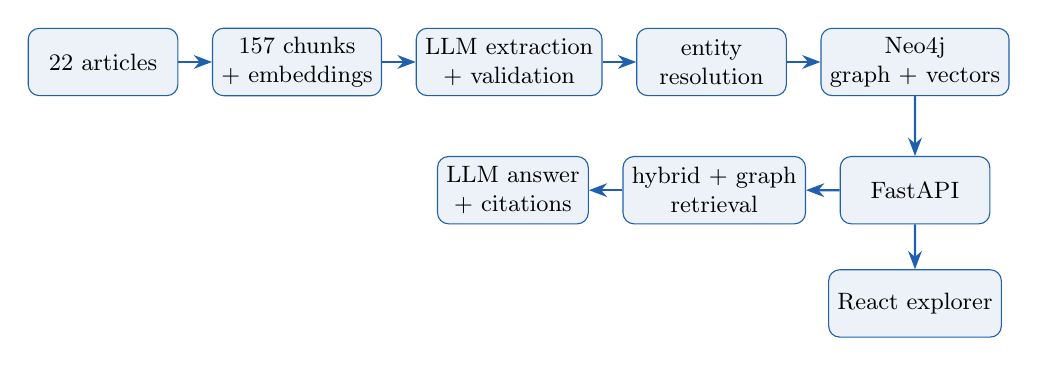
\begin{tikzpicture}[
      box/.style={draw=midblue, rounded corners, fill=midblue!8, minimum width=2.0cm,
                  minimum height=0.9cm, align=center, font=\small},
      arr/.style={-{Stealth}, midblue, thick}, node distance=0.45cm, scale=0.95, transform shape]
    \node[box] (docs) {22 articles};
    \node[box, right=of docs] (chunks) {157 chunks\\+ embeddings};
    \node[box, right=of chunks] (extract) {LLM extraction\\+ validation};
    \node[box, right=of extract] (resolve) {entity\\resolution};
    \node[box, right=of resolve] (neo) {Neo4j\\graph + vectors};
    \node[box, below=0.8cm of neo] (api) {FastAPI};
    \node[box, left=of api] (retr) {hybrid + graph\\retrieval};
    \node[box, left=of retr] (llm) {LLM answer\\+ citations};
    \node[box, below=0.6cm of api] (ui) {React explorer};
    \draw[arr] (docs) -- (chunks); \draw[arr] (chunks) -- (extract);
    \draw[arr] (extract) -- (resolve); \draw[arr] (resolve) -- (neo);
    \draw[arr] (neo) -- (api); \draw[arr] (api) -- (ui);
    \draw[arr] (api) -- (retr); \draw[arr] (retr) -- (llm);
  \end{tikzpicture}
  \vspace{10pt}
  \begin{itemize}\small
    \item Ingestion is \hl{idempotent and cached}: a re-run makes 0 API calls
    \item Result: \hl{726 entities, 585 relations}, every edge knows its source chunks
  \end{itemize}
\end{frame}

%-------------------------------------------------------------
\begin{frame}{Live demo}
  \begin{columns}[T]
    \begin{column}{0.5\textwidth}
      \small
      \begin{enumerate}
        \item Insights: influential owners, communities
        \item Entity card: BAWAG's ownership history
        \item Connect: ÖGB $\leftrightarrow$ GoldenTree
        \item Connect: Refco $\leftrightarrow$ Cerberus
        \item Ask: \emph{Who have been the owners of BAWAG over time?}
        \item Ask: \emph{How is BayernLB connected to Addiko Bank?}
      \end{enumerate}
    \end{column}
    \begin{column}{0.5\textwidth}
      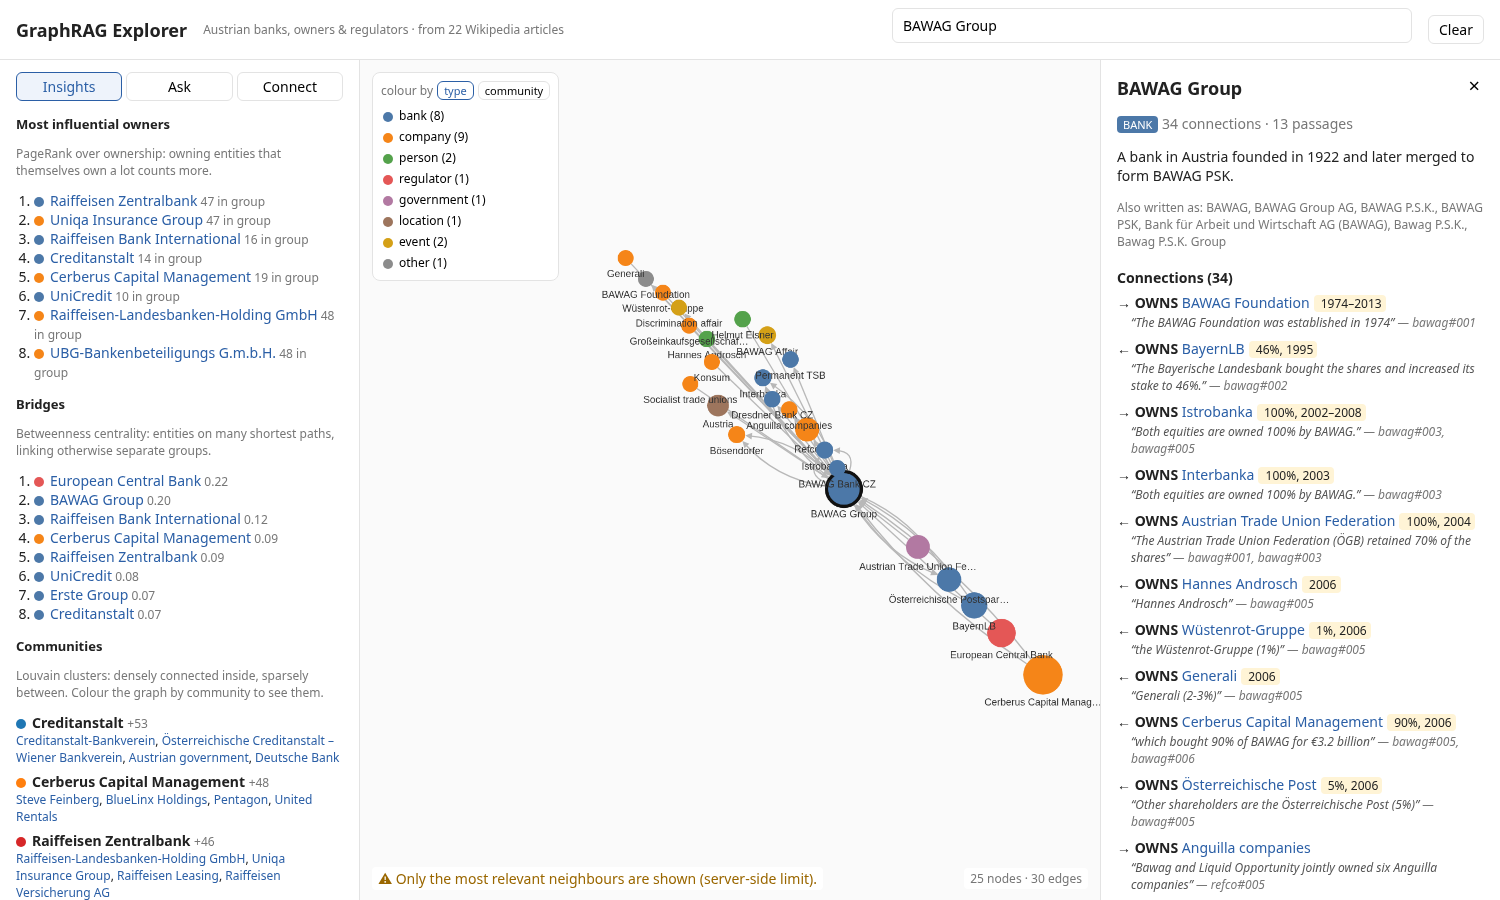
\includegraphics[width=\linewidth]{img/2_bawag.png}
    \end{column}
  \end{columns}
\end{frame}

%-------------------------------------------------------------
\begin{frame}{Extraction: the LLM proposes, code verifies}
  \begin{itemize}
    \item One LLM call per chunk, \hl{Pydantic schema} as structured output
    \item Closed type lists: 8 entity types, 9 relation types
    \item One \hl{canonical direction}: ``A is a subsidiary of B'' becomes \texttt{B OWNS A}
    \item Each item validated on its own: one bad relation does not drop the chunk
    \item \hl{Grounding check}: the evidence quote must be supported by the chunk
  \end{itemize}
  \story{exact-substring grounding rejected 73 relations, \textasciitilde70 of them valid
    (quotes with ``\ldots''). Word-level support: 1 left, and it still catches
    the model dropping umlauts (``\"Osterreichische'' $\rightarrow$ ``sterr ischische'').}
\end{frame}

%-------------------------------------------------------------
\begin{frame}{Entity resolution: false merges are worse than splits}
  \begin{itemize}
    \item Normalise: case, accents, \texttt{\"o}$\rightarrow$\texttt{oe}, legal suffixes (AG, GmbH, a.s.)
    \item Then a \hl{curated alias file}: every merge is explicit and reviewable
    \item Type by majority vote (the LLM says BANK once, COMPANY once)
    \item In a bank, merging two ``Raiffeisen \ldots'' would \hl{invent ownership}
  \end{itemize}
  \story{the key chain ÖGB $\rightarrow$ BAWAG $\leftarrow$ Cerberus was broken: the LLM wrote
    ``Cerberus'' and ``ÖGB'' in one chunk, full names in others. Also: ``Ceberus'' is a typo
    in Wikipedia itself.}
\end{frame}

%-------------------------------------------------------------
\begin{frame}{Retrieval: graph mode}
  \begin{enumerate}
    \item \hl{Hybrid search}: vector + fulltext, fused with Reciprocal Rank Fusion (ranks, not scores)
    \item \hl{Seeds}: entities whose names are covered by the question
    \item \hl{Paths} between seeds, then breadth-first expansion with a node limit
    \item Places are never stepping stones (``both are in Vienna'')
    \item Chunks behind the edges + reranker; \hl{each path edge keeps a slot} for its evidence
    \item Answer with citations; code removes citations of unseen passages
  \end{enumerate}
  \story{degree-based hub filtering blocked the main banks: here the high-degree nodes
    \emph{are} the answer. Type (location) was the right signal.}
\end{frame}

%-------------------------------------------------------------
\begin{frame}{Discovery features}
  \begin{itemize}
    \item \hl{Time and stake on edges}: a second, targeted LLM pass (15 calls, about 200 edges)\\
      \small BayernLB 46\% (1995) $\rightarrow$ ÖGB 100\% (2004) $\rightarrow$ Cerberus 90\% (2006) $\rightarrow$ GoldenTree 21.8\%
    \item \hl{Graph analytics} at ingest (networkx):
      \begin{itemize}\small
        \item PageRank over reversed ownership: who controls the most
        \item Betweenness: bridges between groups (ECB, BAWAG)
        \item Louvain communities: Erste + CEE banks, UniCredit + Bank Austria, \ldots
      \end{itemize}
    \item Path finder without LLM: instant and free
  \end{itemize}
  \story{``SIA'' was a top-5 owner. ``UniCredit sold its \emph{card business} to SIA'' had become
    \texttt{SIA ACQUIRED UniCredit}. One wrong edge distorted a global metric.}
\end{frame}

%-------------------------------------------------------------
\begin{frame}{Engineering for unreliable free-tier APIs}
  \begin{itemize}
    \item Timeouts, retries with backoff, client-side \hl{rate limiter}
    \item \hl{Fallback chain} of models on 503 and on quota errors
    \item \hl{Content-addressed cache}: re-runs are free and reproducible
    \item All-or-nothing writes: a failed run writes nothing and resumes from the cache
    \item API: lifespan-managed resources, dependency injection, request ids, liveness vs readiness
  \end{itemize}
  \story{\texttt{gemini-3.5-flash} allows \hl{20 requests per day}; ingestion needs 160.
    The free tier also counts every text in an embedding batch as one request.}
\end{frame}

%-------------------------------------------------------------
\begin{frame}{Evaluation design}
  \begin{itemize}
    \item 28 questions: 13 multi-hop, 10 lookup, 5 corpus-wide
    \item Built from the \hl{text, not the graph}: otherwise graph mode is graded on its own data
    \item Metrics: recall@8, complete@8, LLM judge, entity recall, latency, tokens
    \item Judge from \hl{another vendor} (Groq) than the answers (Gemini): self-preference bias
    \item \hl{Paired} statistics: bootstrap CIs, McNemar, Wilcoxon
    \item Judge reliability: second judge (Qwen), Cohen's $\kappa$
  \end{itemize}
\end{frame}

%-------------------------------------------------------------
\begin{frame}{Round 1 (original prompt): no measurable difference}
  \centering
  \begin{tabular}{lcc}
    \toprule
    & vector & graph \\
    \midrule
    judge score & 0.91 [0.80, 0.98] & 0.91 [0.84, 0.98] \\
    correct & 24/28 & 23/28 \\
    recall@8 & 0.90 & 0.89 \\
    LLM latency p50 / tokens & 1.7\,s / 2.8k & 2.5\,s / 3.4k \\
    \bottomrule
  \end{tabular}
  \vspace{8pt}
  \begin{itemize}\small
    \item Difference +0.00 [$-$0.05, +0.05], McNemar p = 1.0
    \item \hl{Ceiling effect}: generated questions name their entities, vector finds both passages
    \item Both modes fail on \hl{corpus-wide} questions: top-k cannot collect an aggregation
  \end{itemize}
\end{frame}

%-------------------------------------------------------------
\begin{frame}{Round 2: a pre-registered hard test}
  \begin{itemize}\small
    \item Hypothesis written \hl{before} running: graph wins on connection questions
    \item 8 questions ``How is A connected to C?'', the bridge named nowhere
    \item Prompt fix evaluated only on these new questions: \hl{no tuning on the test set}
  \end{itemize}
  \centering\small
  \begin{tabular}{lcc}
    \toprule
    & vector & graph \\
    \midrule
    judge score & 0.38 & 0.44 \\
    correct & 3/8 & 2/8 \\
    recall@8 & 0.56 & 0.50 \\
    recall@8 \hl{without reranker} & \hl{0.81} & 0.56 \\
    \bottomrule
  \end{tabular}
  \vspace{6pt}
  \begin{itemize}\small
    \item Difference +0.06 [$-$0.12, +0.25]: \hl{hypothesis not supported}
    \item The reranker hurts connection questions most (vector recall 0.81 $\rightarrow$ 0.56)
    \item Regression check on the old 28: nothing broke (graph 0.93 vs vector 0.91)
    \item Two judges agree on 51/56 + 13/16 answers, Cohen's $\kappa$ = 0.62 / 0.69
  \end{itemize}
\end{frame}

%-------------------------------------------------------------
\begin{frame}{What I learned}
  \begin{columns}[T]
    \begin{column}{0.48\textwidth}
      \hl{Where the graph helps}
      \begin{itemize}\small
        \item Exploration: paths, neighbourhoods, rankings
        \item Explainability: every edge has a source quote
        \item Structure: time and stake on ownership
        \item Errors become visible (SIA, Cerberus)
      \end{itemize}
    \end{column}
    \begin{column}{0.48\textwidth}
      \hl{Where it does not (yet)}
      \begin{itemize}\small
        \item QA accuracy on a small, clean corpus
        \item Missing extractions cap it: ``Addiko was spun off from Hypo'' never became an edge
        \item Global questions need graph queries, not top-k
      \end{itemize}
    \end{column}
  \end{columns}
  \vspace{10pt}
  \centering\small
  A negative result, measured honestly, is still a result.
\end{frame}

%-------------------------------------------------------------
\begin{frame}{Next steps}
  \begin{itemize}
    \item Drop or replace the reranker for graph mode (it is trained on web search queries)
    \item Aggregation mode for corpus-wide questions (graph query instead of top-k)
    \item Better extraction recall: a second pass on chunks with few relations
    \item Timeline filter in the explorer (the data is already there)
    \item In a bank: self-hosted or EU-hosted models, Snowflake as the document source,
          Airflow for scheduled re-ingestion
  \end{itemize}
\end{frame}

%-------------------------------------------------------------
\begin{frame}
  \centering
  \Large Thank you. Questions?
  \vspace{12pt}

  \small Code, evaluation and notes: \texttt{graphRAG-demo} repository
\end{frame}

%-------------------------------------------------------------
\appendix
\begin{frame}{Backup: Ask with highlighted path}
  \centering
  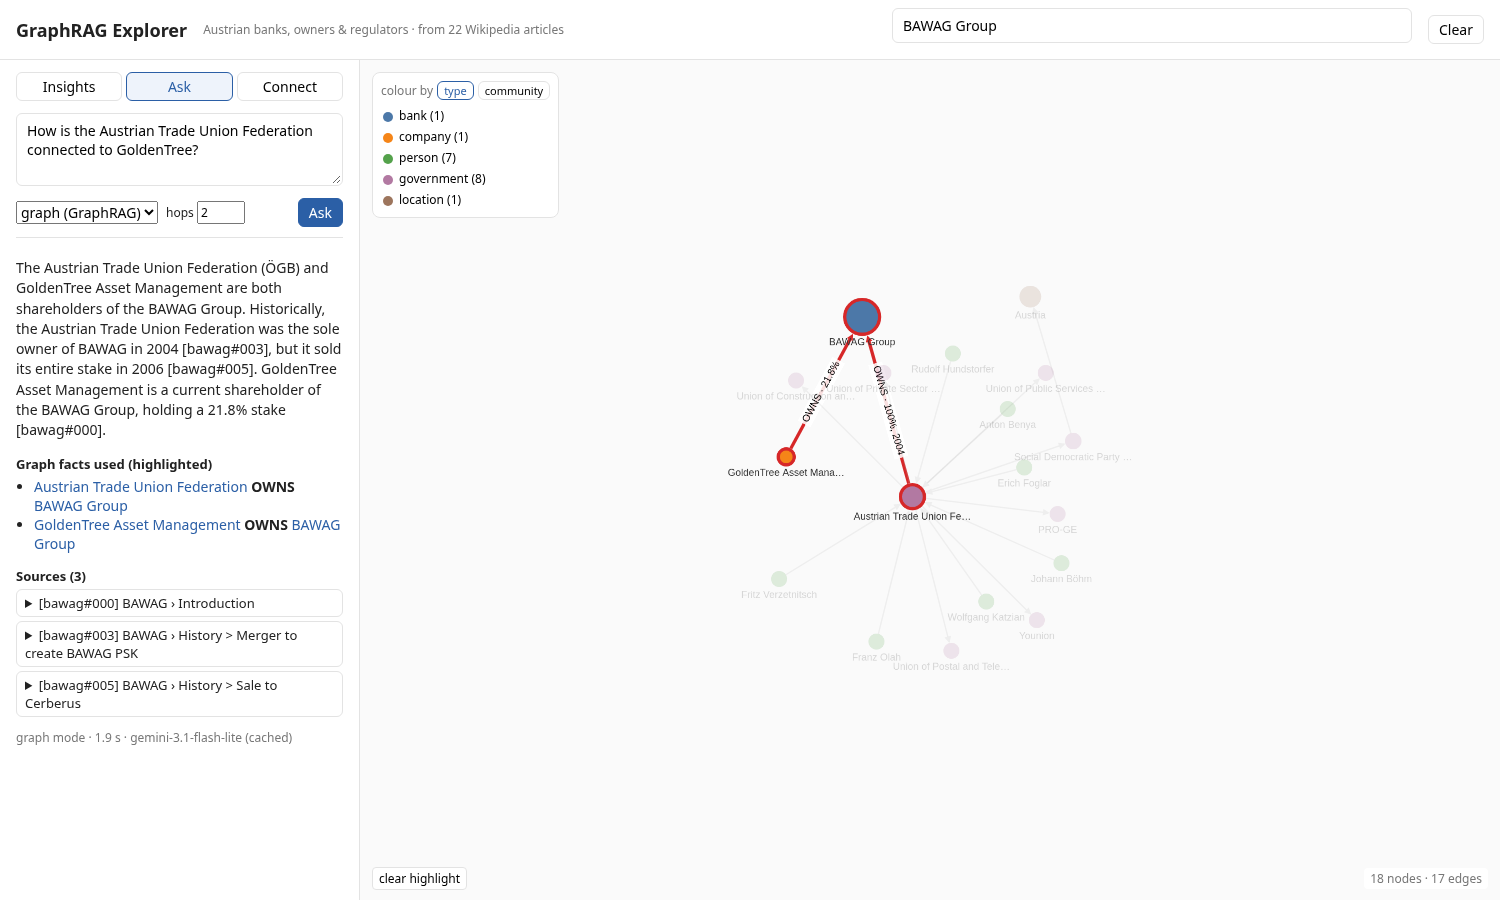
\includegraphics[width=0.85\linewidth]{img/4_ask.png}
\end{frame}

\begin{frame}{Backup: path finder}
  \centering
  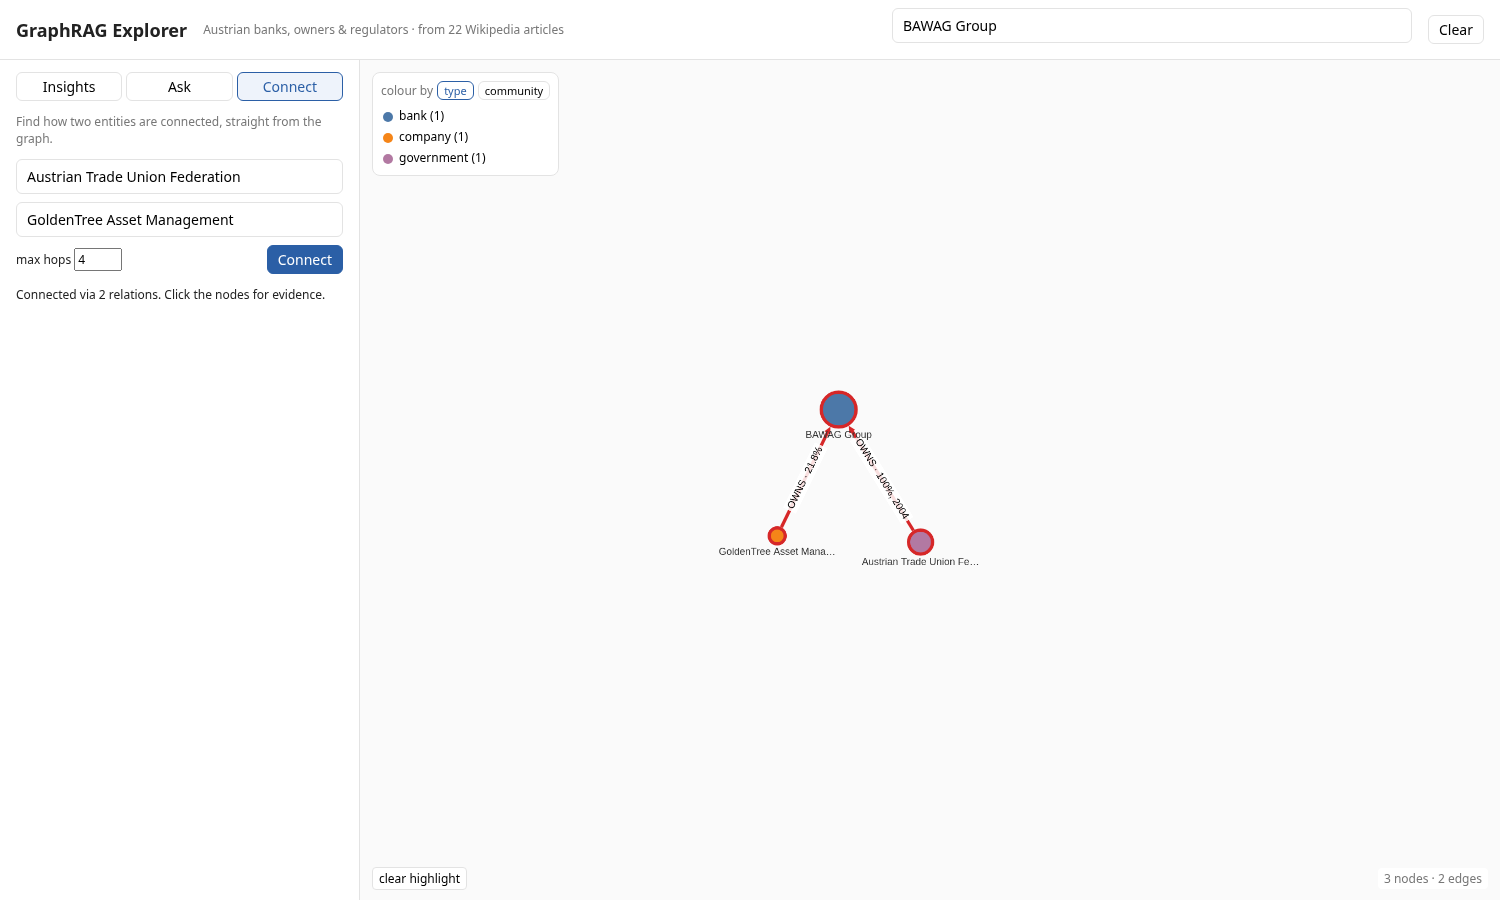
\includegraphics[width=0.85\linewidth]{img/3_path.png}
\end{frame}

\end{document}
